\documentclass[12pt,letterpaper]{article}
\usepackage{graphicx,textcomp}
\usepackage{natbib}
\usepackage{setspace}
\usepackage{fullpage}
\usepackage{color}
\usepackage[reqno]{amsmath}
\usepackage{amsthm}
\usepackage{fancyvrb}
\usepackage{amssymb,enumerate}
\usepackage[all]{xy}
\usepackage{endnotes}
\usepackage{lscape}
\newtheorem{com}{Comment}
\usepackage{float}
\usepackage{hyperref}
\newtheorem{lem} {Lemma}
\newtheorem{prop}{Proposition}
\newtheorem{thm}{Theorem}
\newtheorem{defn}{Definition}
\newtheorem{cor}{Corollary}
\newtheorem{obs}{Observation}
\usepackage[compact]{titlesec}
\usepackage{dcolumn}
\usepackage{tikz}
\usetikzlibrary{arrows}
\usepackage{multirow}
\usepackage{xcolor}
\newcolumntype{.}{D{.}{.}{-1}}
\newcolumntype{d}[1]{D{.}{.}{#1}}
\definecolor{light-gray}{gray}{0.65}
\usepackage{url}
\usepackage{listings}
\usepackage{color}
\usepackage{amsmath} 

\definecolor{codegreen}{rgb}{0,0.6,0}
\definecolor{codegray}{rgb}{0.5,0.5,0.5}
\definecolor{codepurple}{rgb}{0.58,0,0.82}
\definecolor{backcolour}{rgb}{0.95,0.95,0.92}

\lstdefinestyle{mystyle}{
	backgroundcolor=\color{backcolour},   
	commentstyle=\color{codegreen},
	keywordstyle=\color{magenta},
	numberstyle=\tiny\color{codegray},
	stringstyle=\color{codepurple},
	basicstyle=\footnotesize,
	breakatwhitespace=false,         
	breaklines=true,                 
	captionpos=b,                    
	keepspaces=true,                 
	numbers=left,                    
	numbersep=5pt,                  
	showspaces=false,                
	showstringspaces=false,
	showtabs=false,                  
	tabsize=2
}
\lstset{style=mystyle}
\newcommand{\Sref}[1]{Section~\ref{#1}}
\newtheorem{hyp}{Hypothesis}



\begin{document}
	
\title{\textbf{Harnessing Backlash: How Leaders Can Benefit from Antagonizing Foreign Actors}}
\author{Kelly Matush \\ \textit{Florida State University, Tallahassee, FL, USA} \\ https://doi.org/10.7910/DVN/KMDXD7 \\ Harvard Dataverse, V1 \\ \and Replication: Yana Konshyna}
\date{\today}
	
	\maketitle 
	
\textbf{How Leaders Can Benefit from Antagonizing Foreign Actors? }\\

International public diplomacy is generally understood as an attempt to increase foreign goodwill and cooperation. \\

The study of diplomacy has largely focused on states’ ability to use “cheap talk” - which does not have any inherent costs for the speaker - to communicate with or manipulate their international negotiating partners, in spite of strong incentives to misrepresent their interests. These studies are unified by their assumption that public diplomacy is intended to increase positive foreign opinion for the state or the state’s preferred policies.\\

While diplomats nearly always claim to be seeking attraction, leaders also commonly elicit negative reactions from foreign publics. To understand this phenomenon, it is necessary to consider alternative goals for actions that look like public diplomacy but have the opposite effect.\\

This paper argues that intentionally provoking a backlash from a valuable foreign actor, leaders can exchange foreign condemnation for an increase in domestic support. Author refer to this as “strategic antagonism”. \\


\textbf{Why?}\\

A new mechanism through which agency loss can result in noncooperative international outcomes that is distinct from the logic of diversionary war. Rather than generating an immediate military threat that evokes nationalism and unites domestic support, leaders can use strategic antagonism to pay a cost in terms of future international cooperation in order to signal commitment to a policy preferred by a specific domestic constituency.\\

With the rise of populism around the globe, the use of strategic antagonism may become an even more fruitful tool as leaders try to signal their “outsider” credentials and convince voters that they do not conduct “politics as usual". \\

\textbf{Hypothesis}\\

Leaders can intentionally provoke a foreign backlash to gain domestic support, particularly when domestic audiences have policy preferences opposing those of the foreign target. \\

\textbf{Case}\\

In 2015, Israeli Prime Minister Benjamin Netanyahu traveled to the United States to oppose a multilateral agreement with Iran, only to infuriate the Obama administration and polarize US support for Israel. Although risky, Netanyahu’s strategic antagonism appears to have paid large dividends, as he won an extremely tight election the following week and was successful in forming a right-wing coalition government.\\

\textbf{Data}\\

Responses from individuals surveyed just before and just after Netanyahu’s visit to show that the speech had the predicted effect on public opinion within key subsets of both the Israeli and US publics. \\

\vspace{0.1cm}
\noindent \texttt{data\_US}: 4866 obs. of 12 variables. Gallup and Pew each ran one survey in the weeks before the speech and in the weeks after. Data are from the Roper iPoll Center.\\

\vspace{0.1cm}
\noindent \texttt{data\_INES}: 174 obs. of 7 variables. Data are from the 2015 Israel National Election Survey.
\vspace{0.1cm}
	\lstinputlisting[language=R, firstline=11,lastline=11]{Replication_YK_23359606.R} 
	
	\begin{figure}[H]
	\centering
	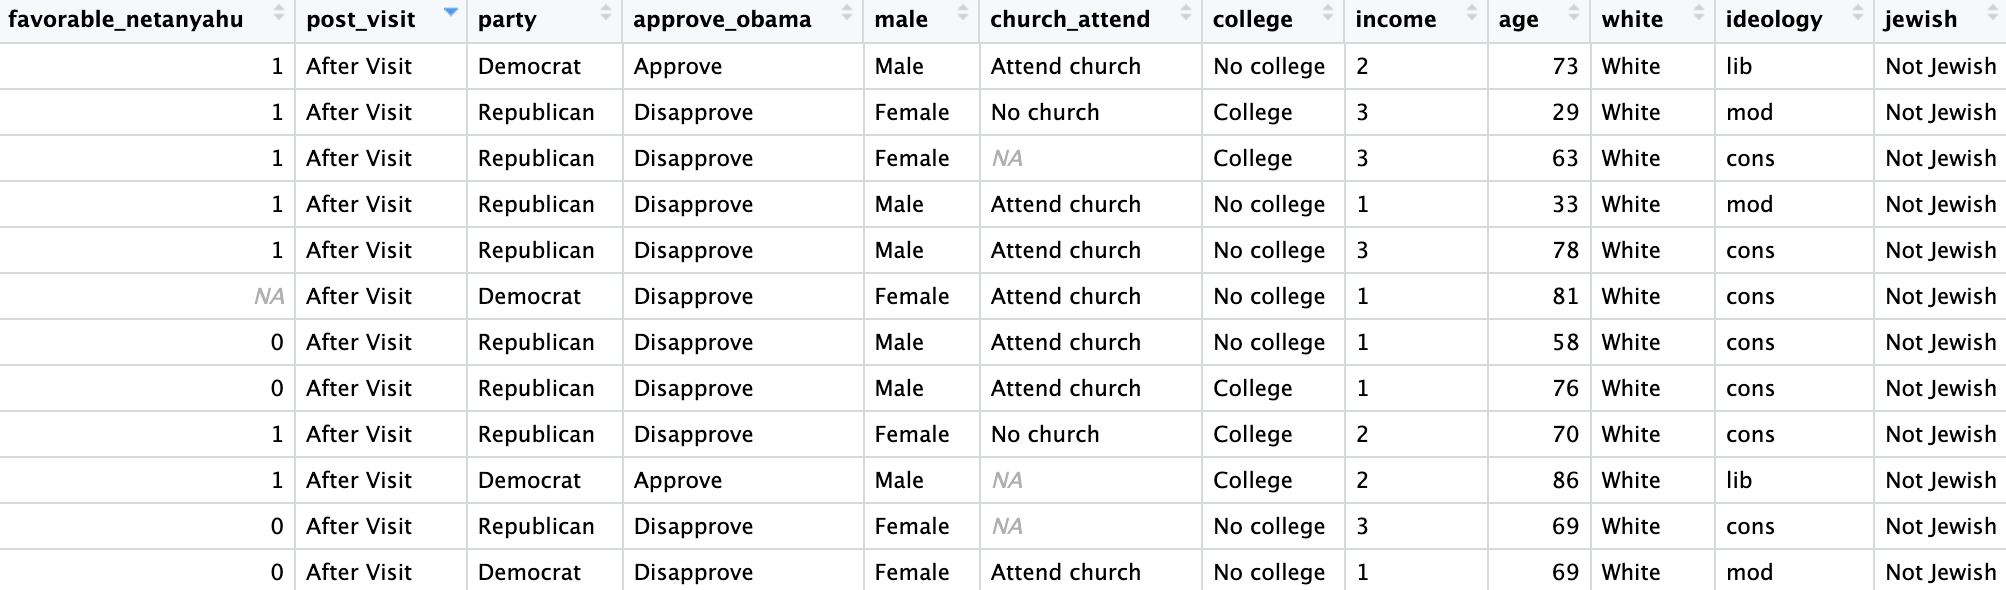
\includegraphics[width=1.0\textwidth]{Images/Image1.png}
	\refstepcounter{figure} 
	\label{fig:your_figure_label} 
%	\textbf{Figure~\thefigure.}
	%	\label{fig:figure1}
\end{figure}

\textbf{Model 1: American public opinion }\\
Independent variable: IV (Democrat), After speech, X (vector of control variables)  \\
Dependent variable: Netanyahu Approval \\

\textbf{Model 2: American Democrats opinion}\\
Independent variable: IV (Approves of Obama), After speech, X (vector of control variables) \\
Dependent variable: Netanyahu Approval  \\

	\lstinputlisting[language=R, firstline=42,lastline=42]{Replication_YK_23359606.R} 
	
		\begin{figure}[H]
		\centering
		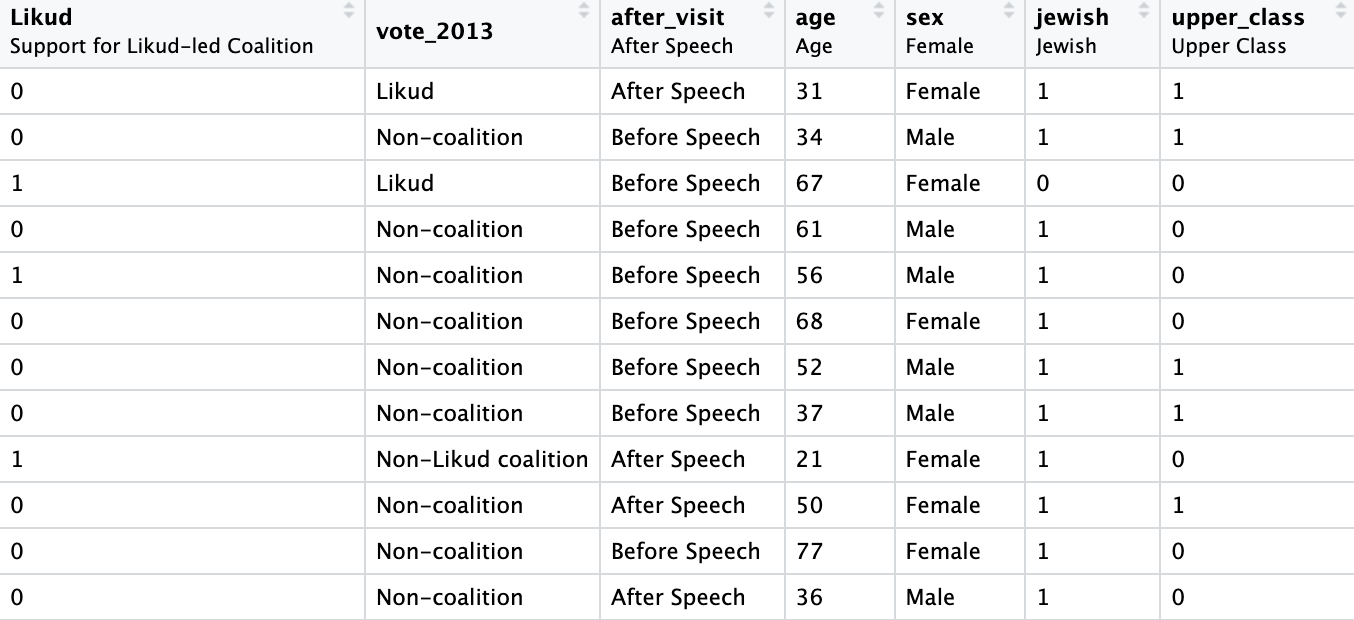
\includegraphics[width=1.0\textwidth]{Images/Image2.png}
		\refstepcounter{figure} 
		\label{fig:your_figure_label} 
%		\textbf{Figure~\thefigure.}
		%	\label{fig:figure1}
	\end{figure}

\textbf{Model 3: Israeli public opinion}\\
Independent variable: Coalition vote in 2013, After speech, X (vector of control variables)  \\
Dependent variable: Support Likud Coalition\\

\textbf{Assumptions for Model 3:}
\begin{itemize}
	\item \textbf{Linearity:} The relationship between X and the mean of Y is linear.
	\item \textbf{Homoscedasticity:} The variance of residual is the same for any value of X.
	\item \textbf{Independence:} Observations are independent of each other.
	\item \textbf{Normality:} For any fixed value of X, Y is normally distributed.
\end{itemize}
	

	\begin{center}
		\noindent \textbf{Model 1 and Model 2}
	\end{center}
	
A probit model was used to analyze the change in American public opinion before and after Netanyahu’s speech. The dependent variable \texttt{Netanyahu Approval} is a dummy variable indicating whether the respondents reported a favorable opinion of Netanyahu. Two key independent variables \texttt{IV} representing the subset of Americans that expected to be alienated by Netanyahu’s speech: 1) a categorical variable indicating the respondent’s party, the key subgroup being Americans who identify as Democrats (Democrat), and 2) a dummy variable indicating whether the respondent expressed approval of President Obama (Approves of Obama). These variables are only correlated at 0.43, indicating that they are capturing significantly different subsets of the American public. Author interacted these \texttt{IV}s with a dummy variable indicating whether the respondent was surveyed after Netanyahu’s speech (\texttt{After Speech}).
	
%		\vspace{0.5cm}
	\begin{center}
		\noindent \textbf{Model 1 - American Public Opinion}
	\end{center}
	
%	\vspace{0.5cm}
	\noindent The estimating equation:
	\begin{equation}
		\text{Netanyahu Approval} \sim \beta_{0} + \beta_{1} \times \text{After Speech} + \beta_{2} \times \text{IV} + \beta_{3} \times \text{After Speech} \times \text{IV} + \beta_{4} \times X,
	\end{equation}
	
	\noindent where \texttt{X} is a vector of control variable and independent variable \texttt{IV} is Democrat.
	
	\vspace{0.5cm}
	\noindent  Running probit regression:
	\lstinputlisting[language=R, firstline=14,lastline=14]{Replication_YK_23359606.R} 
	
	\begin{figure}[H]
		\centering
		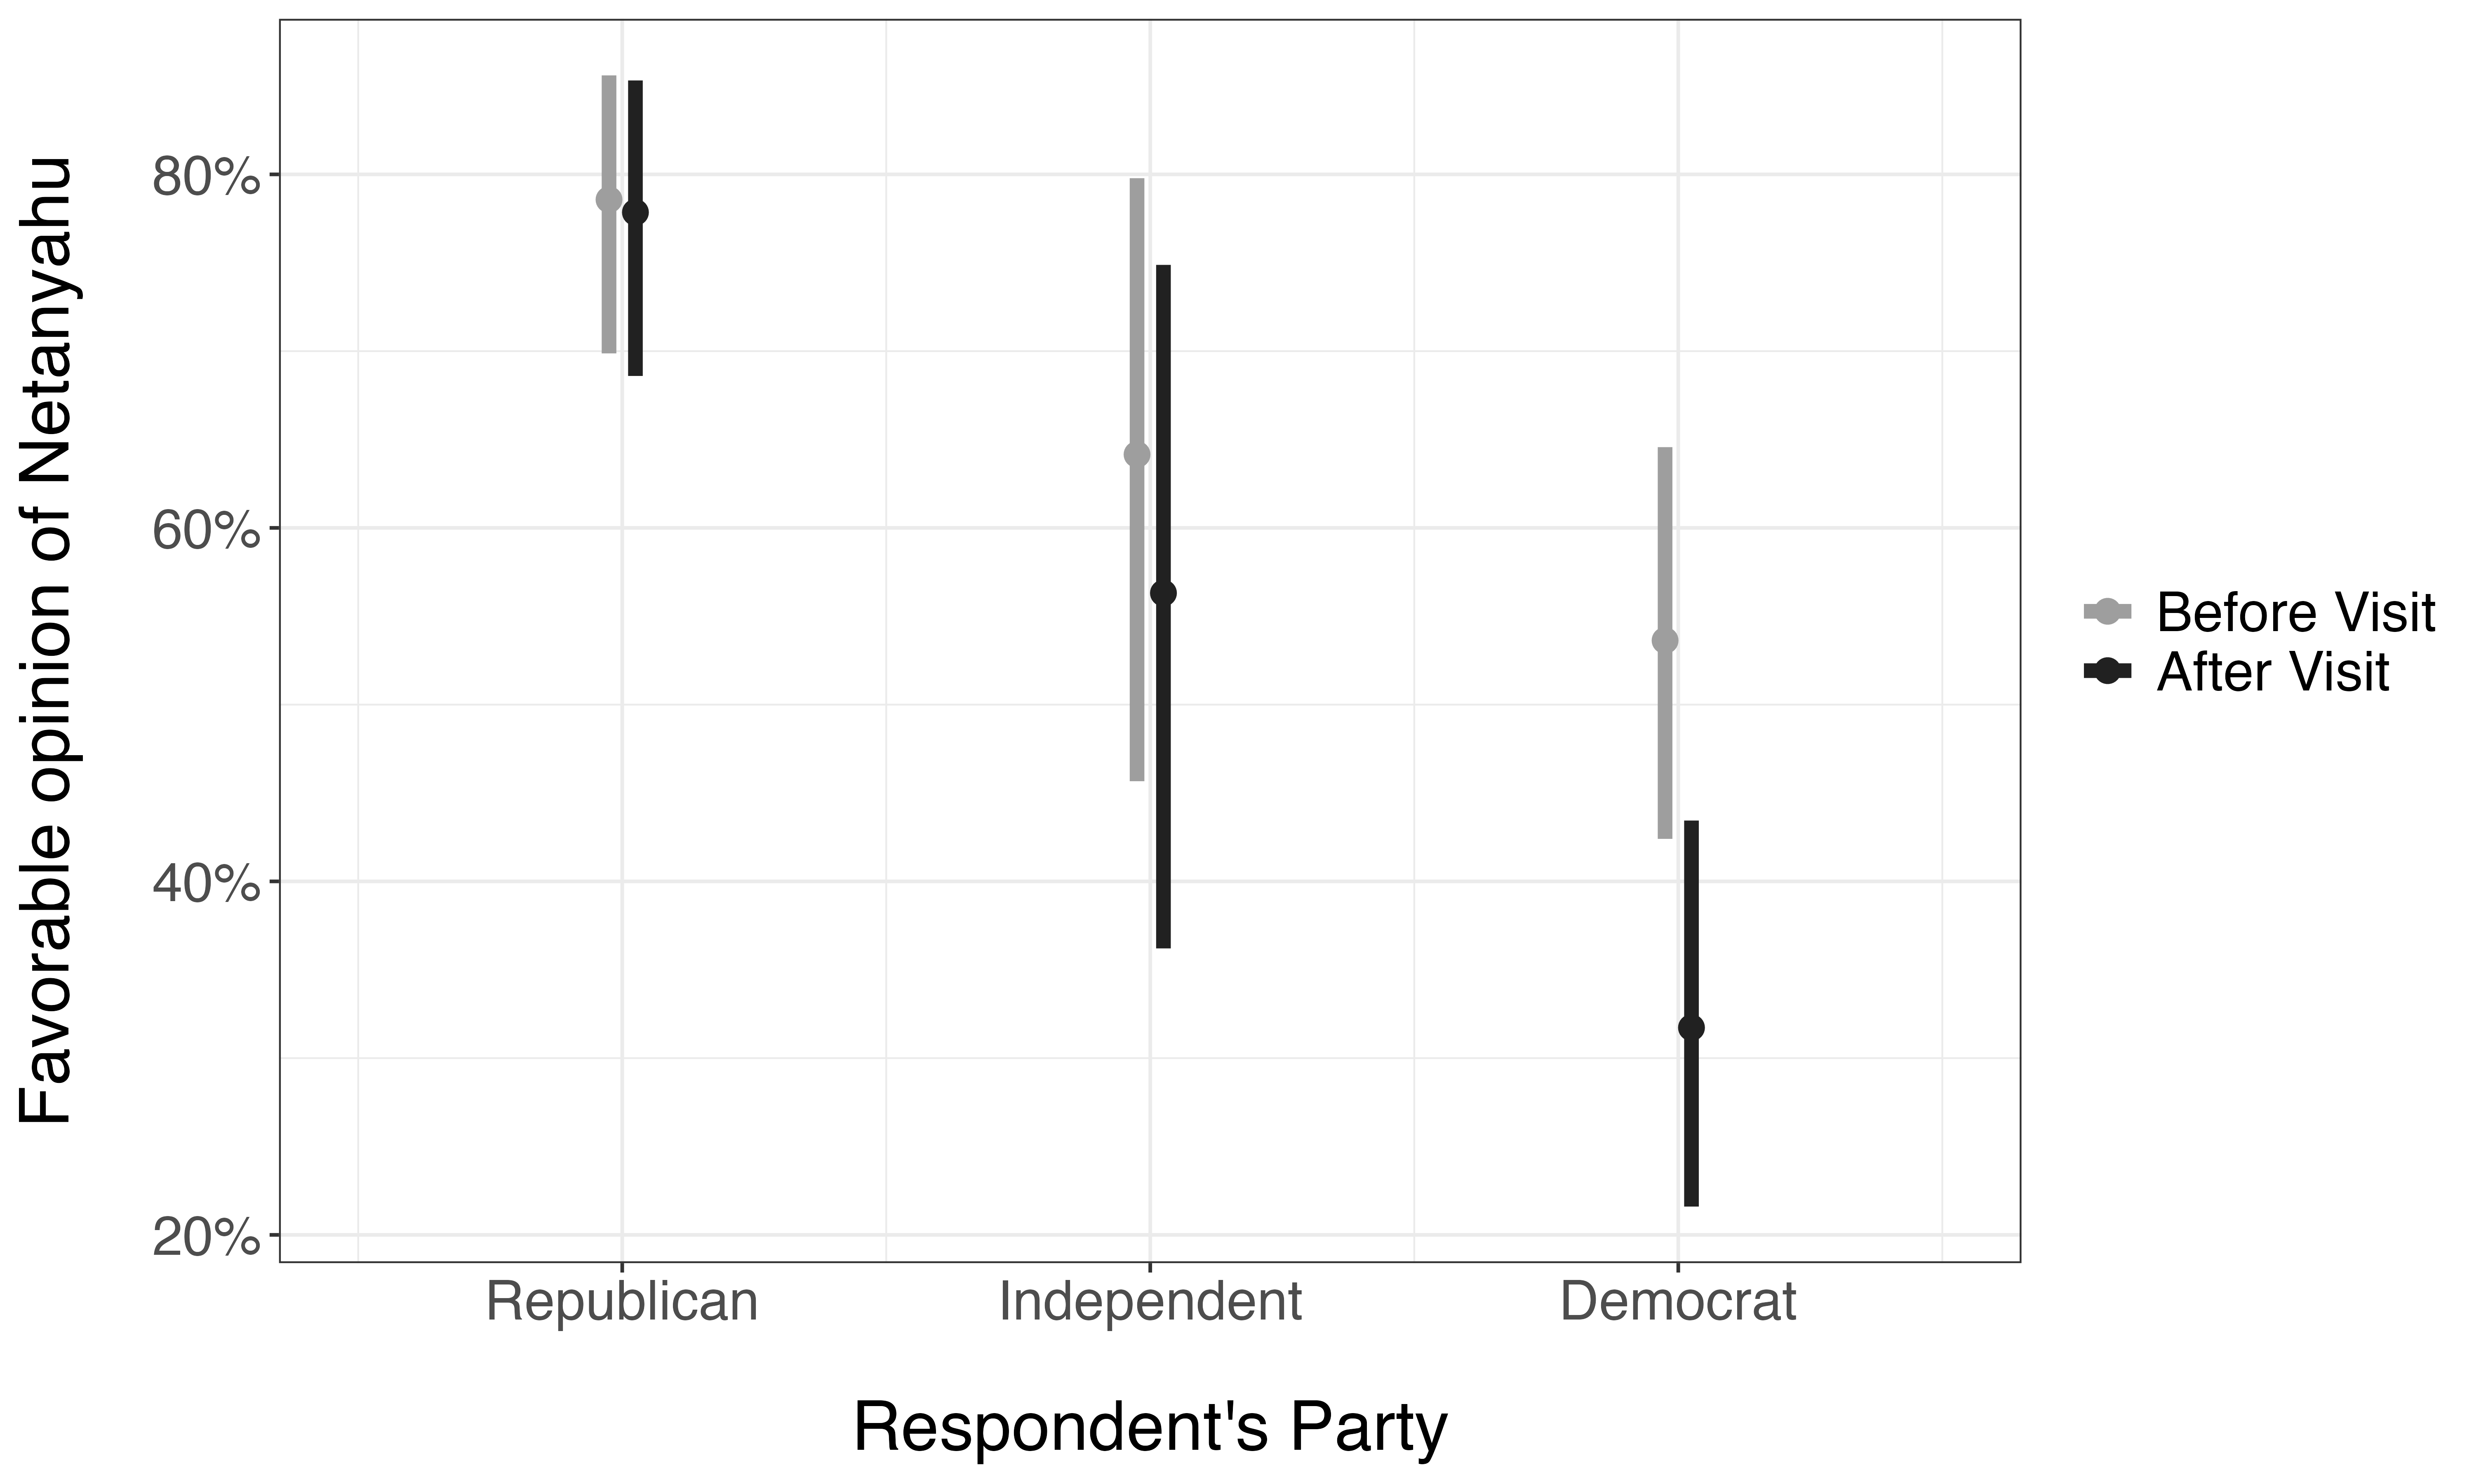
\includegraphics[width=1.0\textwidth]{figures_rep/Figure1.png}
		  \refstepcounter{figure} 
		      \label{fig:your_figure_label} 
		  \textbf{Figure~\thefigure.}
	%	\label{fig:figure1}
	\end{figure}
	
Model 1 shows that average American opinion of Netanyahu became more unfavorable following his speech. Republicans did not significantly change their approval of Netanyahu, while Democrats decreased their approval of Netanyahu by 21.1\%. Vertical bars are 95\% confidence intervals. The decrease within Democrats is statistically significant \(p < 0.05\) (Figure 1).
	
%	\vspace{1cm}
\begin{center}
		\noindent \textbf{Model 2 - American Democrats Opinion}
\end{center}

However, Model 2 demonstrates that this movement was much larger among American Democrats.
	
		\vspace{0.5cm}
	\noindent The estimating equation:
	\begin{equation}
		\text{Netanyahu Approval} \sim \beta_{0} + \beta_{1} \times \text{After Speech} + \beta_{2} \times \text{IV} + \beta_{3} \times \text{After Speech} \times \text{IV} + \beta_{4} \times X,
	\end{equation}
	
	\noindent where \texttt{X} is a vector of control variable and independent variable \texttt{IV} is Approves of Obama. 
			\vspace{0.5cm}
	\noindent  Running probit regression: 
	\lstinputlisting[language=R, firstline=28,lastline=28]{Replication_YK_23359606.R} 
	
	\begin{figure}[H]
		\centering
		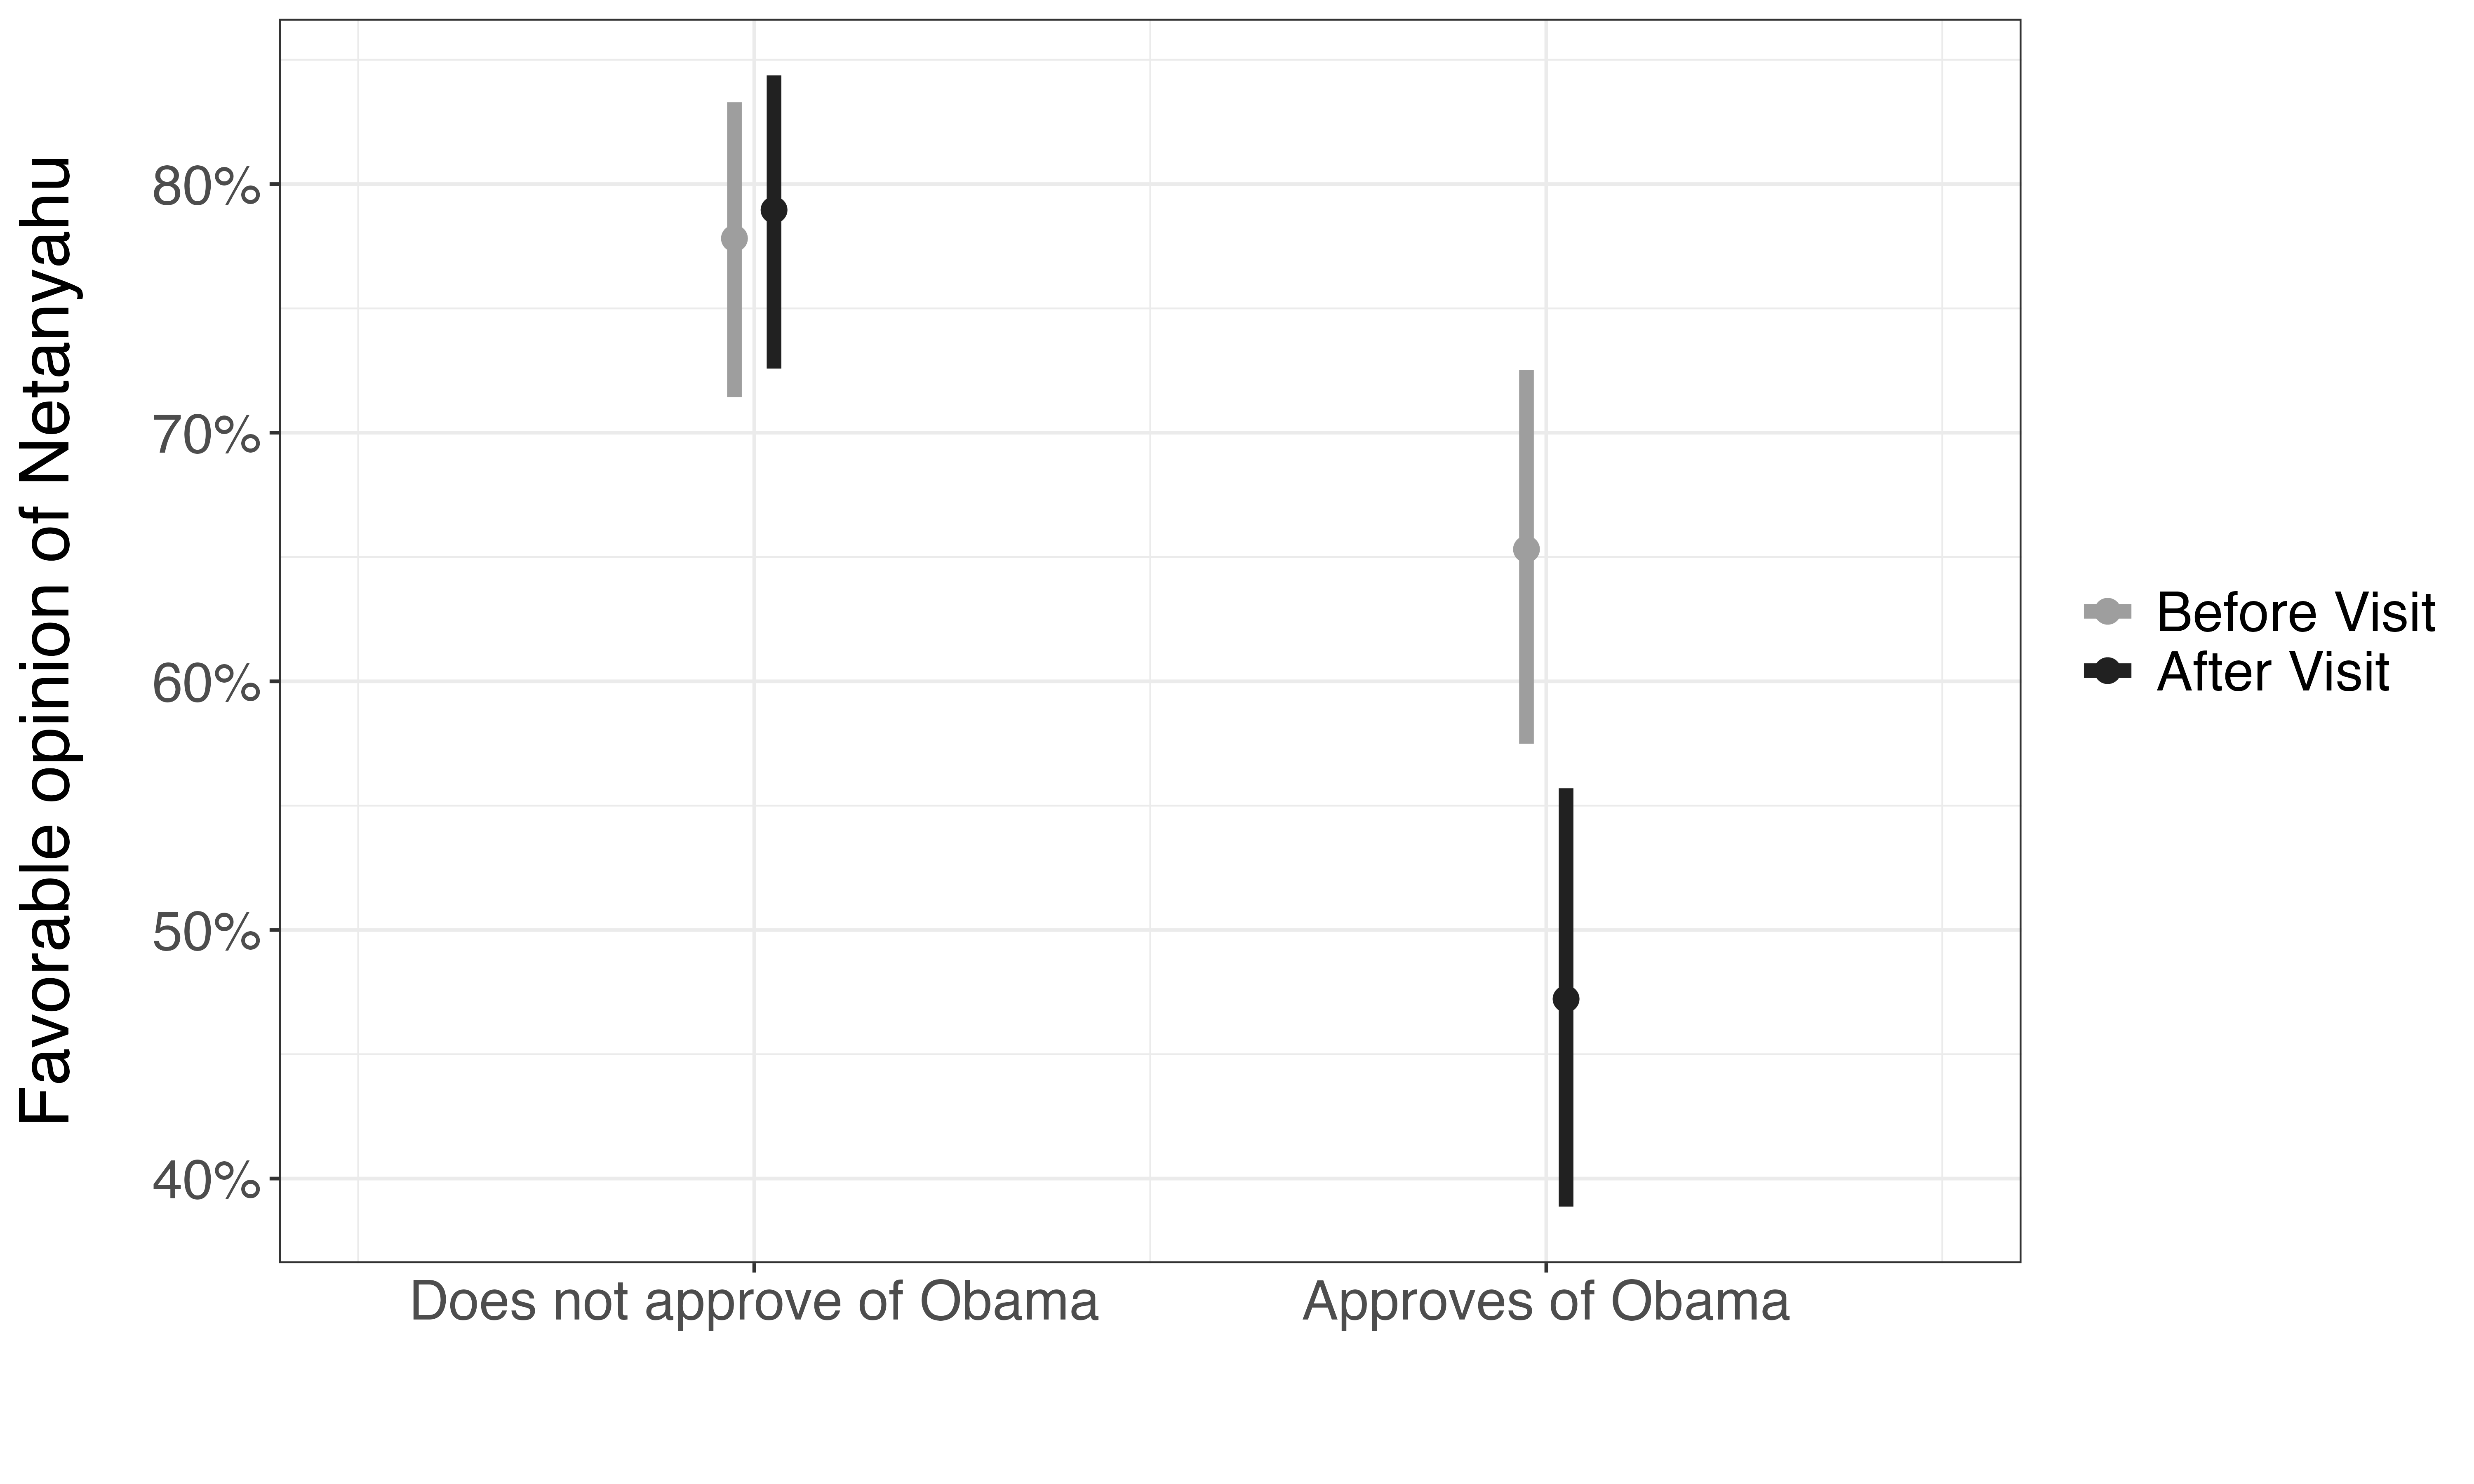
\includegraphics[width=1.0\textwidth]{figures_rep/Figure2.png}
				  \refstepcounter{figure} 
		\label{fig:your_figure_label} 
		\textbf{Figure~\thefigure.}
		\label{fig:figure2}
	\end{figure}
	
Model 2 shows that Americans that did not approve of Obama did not change their favorability towards Netanyahu following his speech, while Americans that approved of Obama decreased their favorability rating of Netanyahu by 17.1\% \(p<0.05\). Vertical bars are 95\% confidence intervals (Figure 2).
	
%	\vspace{1cm}
\begin{center}
		\noindent \textbf{Model 3 - Israeli Public Opinion}
\end{center}

In 2015, Netanyahu was campaigning to form a coalition including right-wing parties: United Torah Judaism, Shas, and Jewish Home. Author examined the relationship between whether a respondent supported one of these parties in the 2013 Knesset election, and whether they express a preference for a coalition led by the Likud. \\

An OLS model was used to analyze the change in Israeli public opinion before and after Netanyahu’s speech. \\
%	\vspace{0.5cm}

\noindent The estimating equation:
	\begin{align}
		\text{Support Likud Coalition} \sim & \, \beta_{0} + \beta_{1} \times \text{After Speech} + \beta_{2} \times \text{Coalition vote in 2013} \nonumber \\
		& + \beta_{3} \times \text{After Speech} \times \text{Coalition vote in 2013} + \beta_{4} \times X,
	\end{align}


\noindent where \texttt{X} is a vector of control variable, \texttt{After Speech}  is a dummy variable indicating whether the respondent was surveyed after Netanyahu’s speech, \texttt{Coalition vote in 2013} is dummy variable indicating whether the respondent supported one of right-wing parties in the 2013 Knesset election.

\vspace{0.5cm}
\noindent  Running OLS regression: 
\lstinputlisting[language=R, firstline=45,lastline=45]{Replication_YK_23359606.R} 

	\begin{figure}[H]
		\centering
		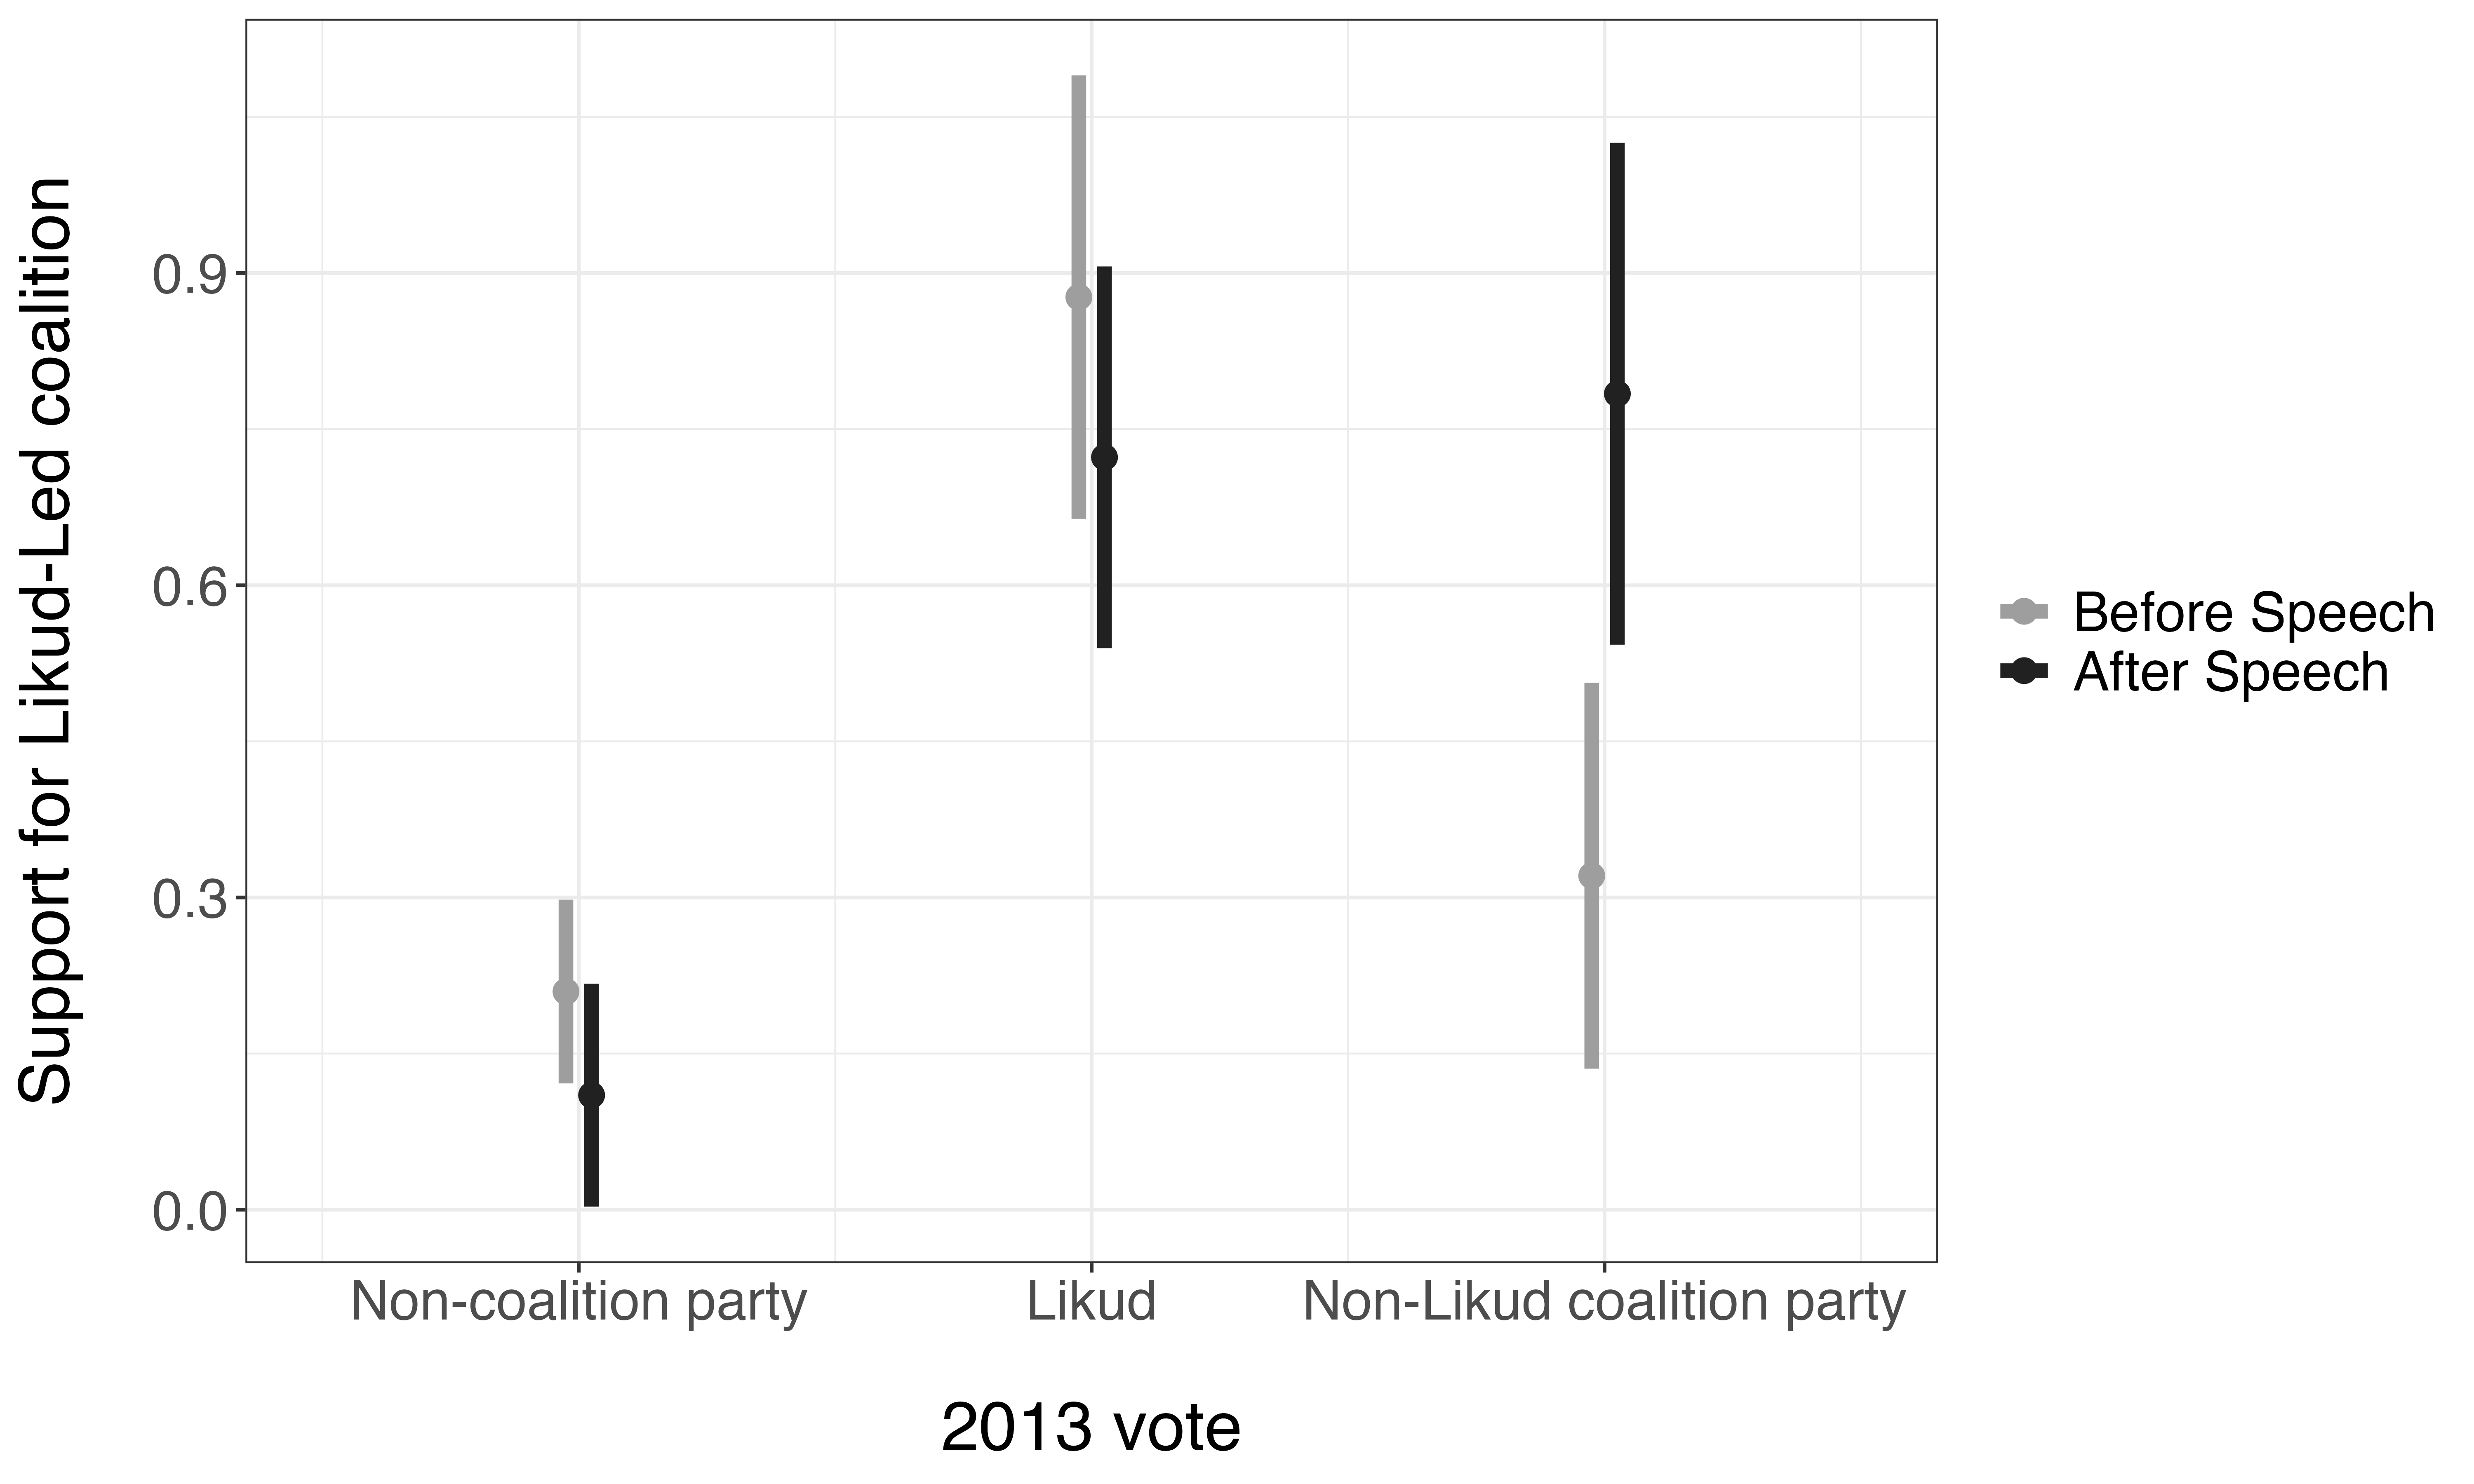
\includegraphics[width=1.0\textwidth]{figures_rep/Figure3.png}
				  \refstepcounter{figure} 
		\label{fig:your_figure_label} 
		\textbf{Figure~\thefigure.}
		\label{fig:figure3}
	\end{figure}
	
Model 3 shows that Israelis who voted for a right-wing coalition party in 2013 increased their support for a Likud-led coalition in the period following Netanyahu’s speech \(p < 0.05\). Vertical bars are 95\% confidence intervals (Figure 3).
	
%	\vspace{1m}
\begin{center}
	\noindent \textbf{Extension: Model 3a - Israeli Public Opinion with and without interaction term}
\end{center}

Interaction terms can make the interpretation of the model coefficients more complex. The effect of one predictor depends on the level of the other variable it interacts with. So, instead multiplicative model I decided to run additive.

	\vspace{0.2cm}
	\noindent  1. Running multiplicative linear Model 3 with interaction term. 
	\lstinputlisting[language=R, firstline=61,lastline=61]{Replication_YK_23359606.R} 

	\vspace{0.2cm}
\noindent  2. Running additive linear Model 3a without interaction term. 
\lstinputlisting[language=R, firstline=66,lastline=66]{Replication_YK_23359606.R} 
		\vspace{0.2cm}

\noindent  3. Printing the estimated coefficients of linear model with and without interaction term for comparison. (\textbf{Table 1.})
\lstinputlisting[language=R, firstline=80,lastline=80]{Replication_YK_23359606.R} 
	\vspace{0.2cm}
	
	\noindent \textbf{Conclusion}: The presence of interaction terms allows for the examination of how the effect of \texttt{vote\_2013} categories on Likud changes before and after the speech (\texttt{after\_visit}). The significant interaction between \texttt{vote\_2013Non-Likud coalitio}n and \texttt{after\_visitAfter Speech} indicates that for voters in the non-Likud coalition, the effect of the speech is important (statistically differantiable from zero), suggesting that these voters' support for Likud changes differently after the speech compared to voters not in this category or time period.
	
			\vspace{0.2cm}
By removing the interaction terms, each predictor's effect is considered independently of the levels of other variables. This means that the Model 3a no longer accounts for the combined effect of voting behavior in 2013 and the timing relative to the speech. This model assumes the effect of voting behavior and the timing of the speech (before/after) on Likud support is constant, not influenced by the combination of these factors.
	
			\vspace{0.2cm}
	\begin{figure}[H]
		\centering
		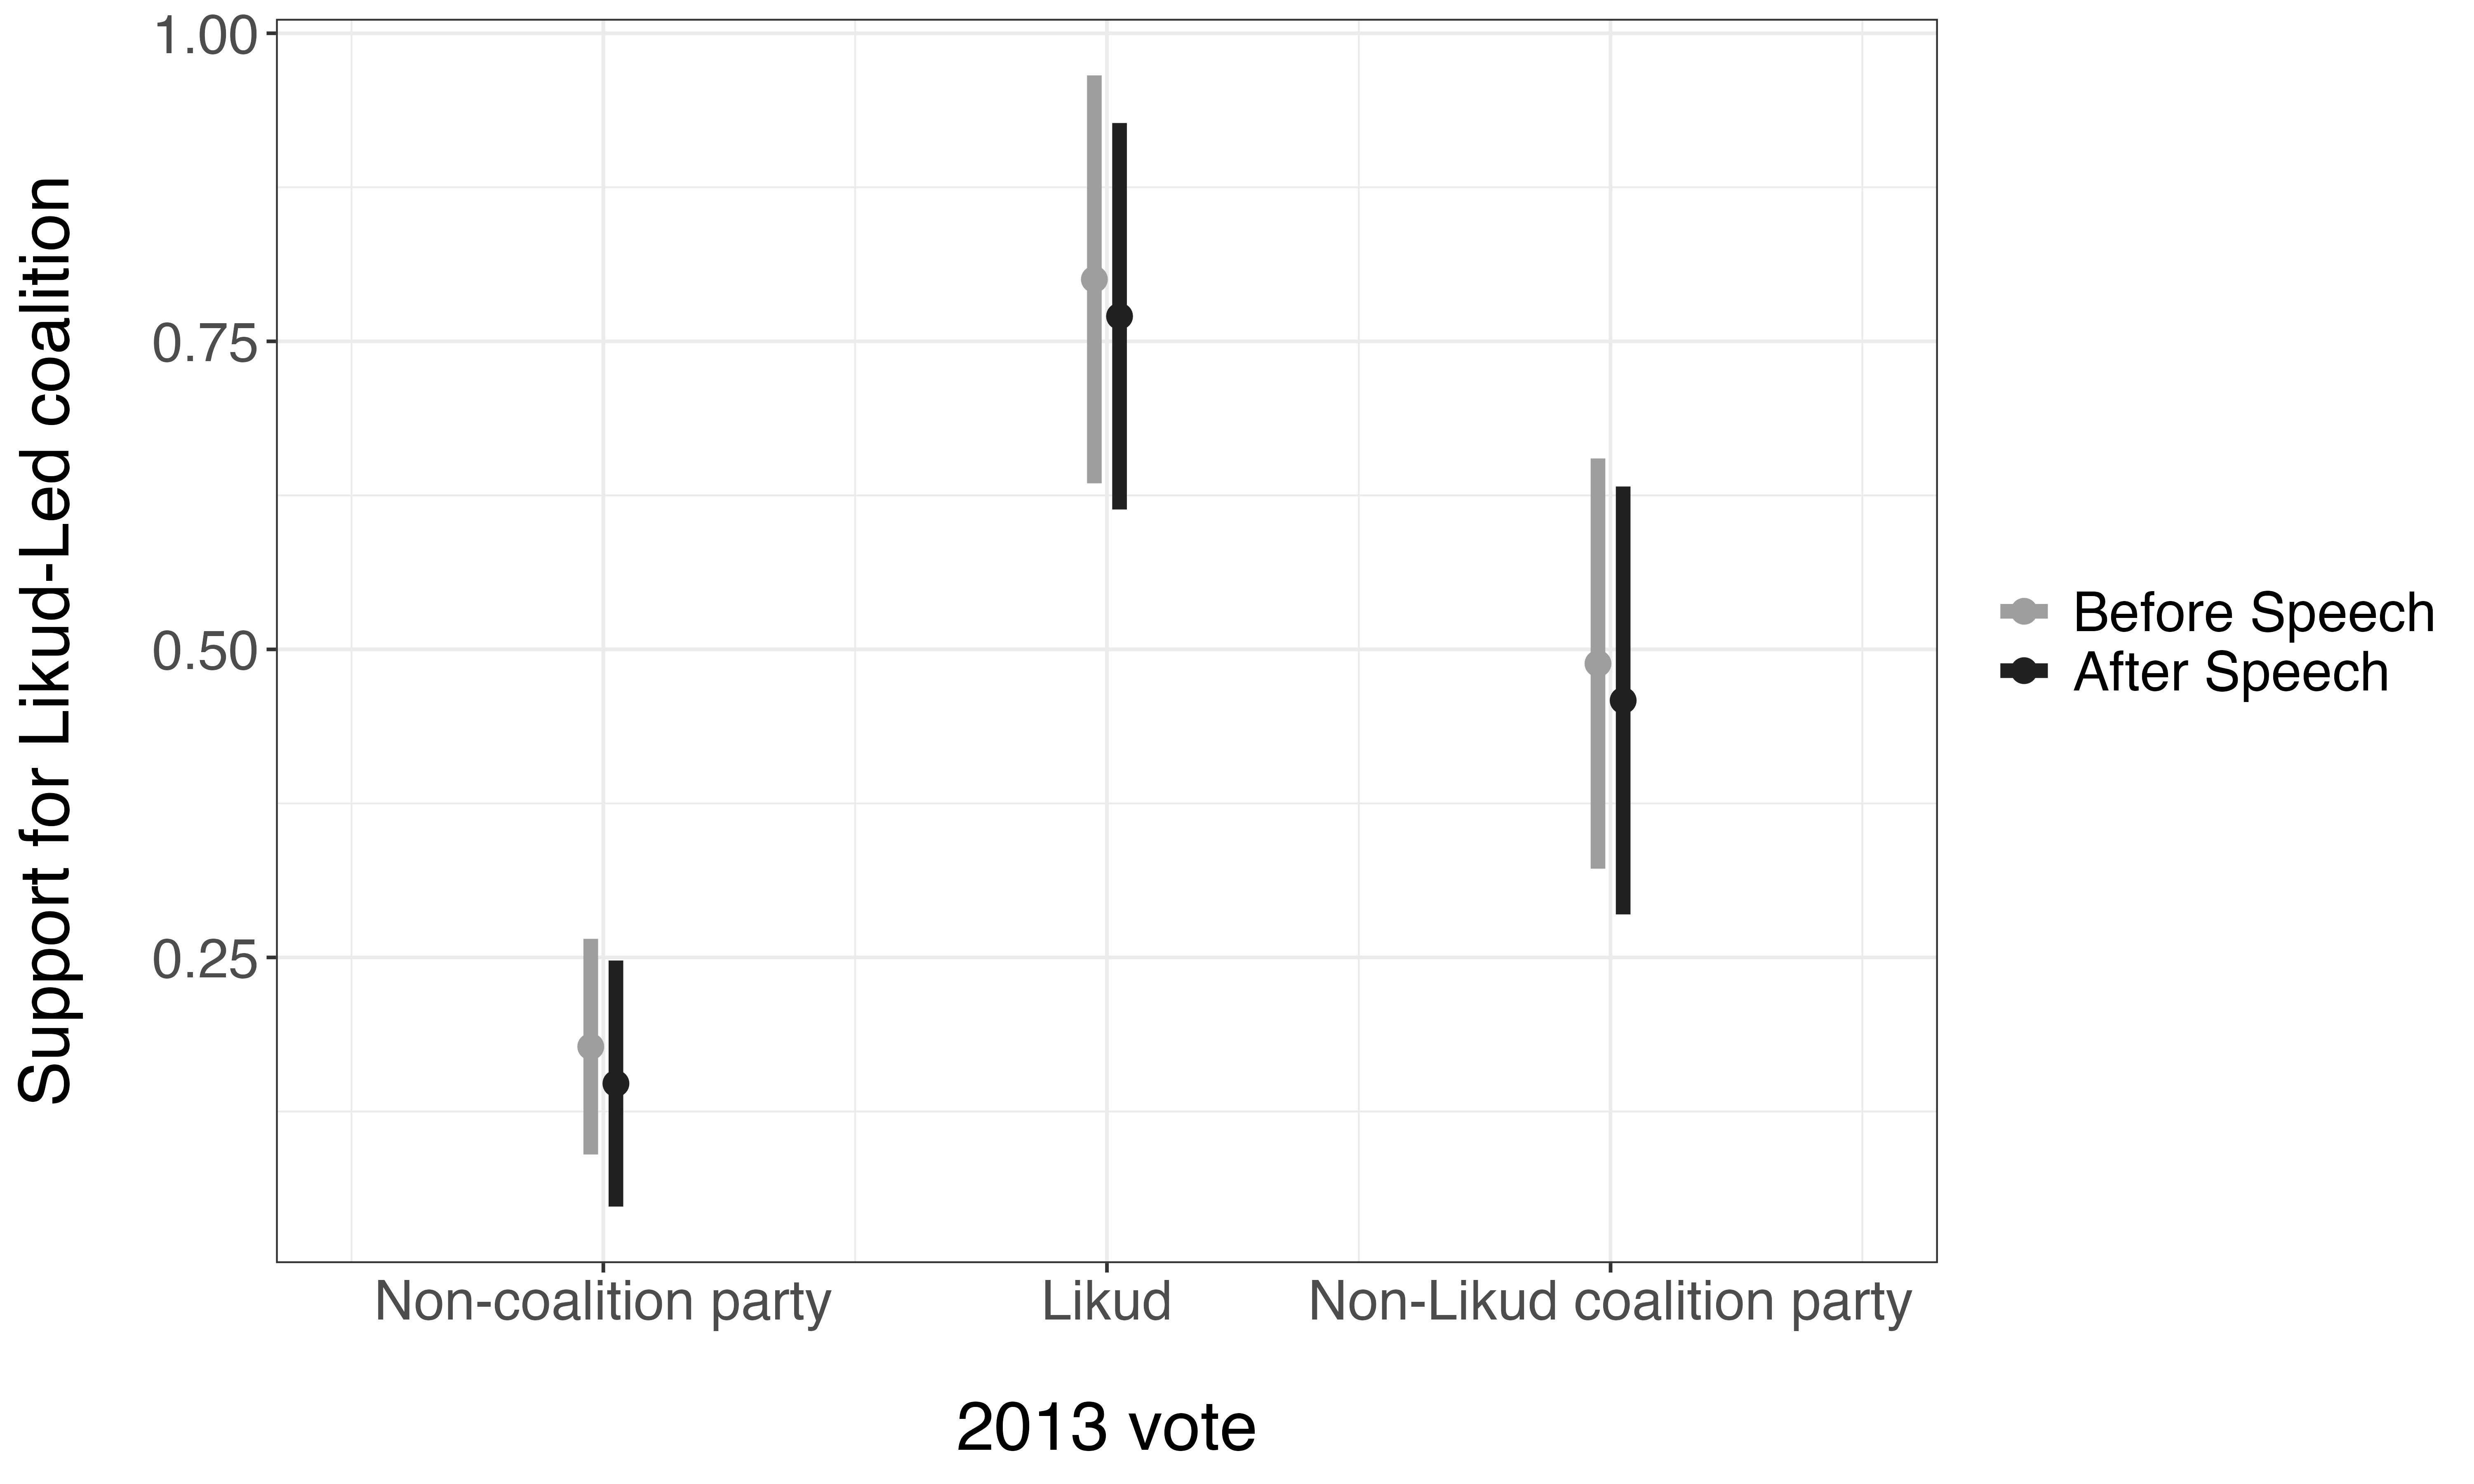
\includegraphics[width=1.0\textwidth]{figures_rep/Figure3a.png}
		\refstepcounter{figure} 
		\label{fig:your_figure_label} 
		\textbf{Figure 3a.}
		\label{fig:figure4}
	\end{figure}
	
The removal of interaction term may overlook important dynamics between the time of the speech and prior voting behavior (Figure 3a). The multiplicative Model 3 captures the unique effect of the speech on changing attitudes towards Likud for different voter groups, which is lost in the additive Model 3a.

	\vspace{0.2cm}
\begin{table}[!htbp] \centering   \caption{Models Comparison}   \label{} \begin{tabular}{@{\extracolsep{5pt}}lcc} \\[-1.8ex]\hline \hline \\[-1.8ex]  & \multicolumn{2}{c}{\textit{Dependent variable:}} \\ \cline{2-3} \\[-1.8ex] & \multicolumn{2}{c}{Likud} \\ \\[-1.8ex] & \textbf{Model 3} & \textbf{Model 3a}\\ \hline \\[-1.8ex]  vote\_2013Likud & 0.667$^{***}$ & 0.623$^{***}$ \\   & (0.126) & (0.090) \\   & & \\  vote\_2013Non-Likud coalition & 0.111 & 0.311$^{***}$ \\   & (0.113) & (0.094) \\   & & \\  after\_visitAfter Speech & $-$0.100 & $-$0.030 \\   & (0.074) & (0.064) \\   & & \\  age & $-$0.005$^{**}$ & $-$0.006$^{***}$ \\   & (0.002) & (0.002) \\   & & \\  sexFemale & 0.035 & 0.051 \\   & (0.062) & (0.063) \\   & & \\  jewish & 0.227$^{***}$ & 0.219$^{**}$ \\   & (0.083) & (0.085) \\   & & \\  upper\_class & $-$0.183$^{**}$ & $-$0.193$^{***}$ \\   & (0.072) & (0.073) \\   & & \\  vote\_2013Likud:after\_visitAfter Speech & $-$0.054 &  \\   & (0.173) &  \\   & & \\  vote\_2013Non-Likud coalition:after\_visitAfter Speech & 0.563$^{***}$ &  \\   & (0.186) &  \\   & & \\  Constant & 0.290$^{***}$ & 0.300$^{***}$ \\   & (0.111) & (0.113) \\   & & \\ \hline \\[-1.8ex] Observations & 166 & 166 \\ R$^{2}$ & 0.384 & 0.345 \\ Adjusted R$^{2}$ & 0.349 & 0.316 \\ Residual Std. Error & 0.379 (df = 156) & 0.389 (df = 158) \\ F Statistic & 10.824$^{***}$ (df = 9; 156) & 11.903$^{***}$ (df = 7; 158) \\ \hline \hline \\[-1.8ex] \textit{Note:}  & \multicolumn{2}{r}{$^{*}$p$<$0.1; $^{**}$p$<$0.05; $^{***}$p$<$0.01} \\ \end{tabular} \end{table} 
	
\end{document}
